
% This LaTeX was auto-generated from an M-file by MATLAB.
% To make changes, update the M-file and republish this document.

\documentclass{article}
\usepackage{graphicx}
\usepackage{color}

\sloppy
\definecolor{lightgray}{gray}{0.5}
\setlength{\parindent}{10pt}
\usepackage[margin=1in]{geometry}

\begin{document}

\title{Dynamical Adaptation in ORNs}
\author{Srinivas Gorur-Shandilya}
\maketitle

    
    
\section*{Does Spike Frequency Adaptation imply Dynamical Adaptation?}

\begin{par}
Liu and Wang's (papers2://publication/uuid/54F8985C-DC25-42D9-AD8B-805EBCD7475F) model of spike frequency adaptation shows some qualitative similarity to ORN response dynamics. Can the mechanics of spike frequency adaptation also give rise to a phenomenon like fast dynamical adaptation?
\end{par} \vspace{1em}

\subsection*{Contents}

\begin{itemize}
\setlength{\itemsep}{-1ex}
   \item Response properties of Model Neuron
   \item Response to exponentiated Gaussian stimuli
   \item Does this show the signature of fast adaptation?
\end{itemize}


\subsection*{Response properties of Model Neuron}

\begin{par}
In this plot, a Liu-Wang model neuron is simulated using parameters very close to what they use in the paper. The parameters are:
\end{par} \vspace{1em}

        \color{lightgray} \begin{verbatim}        Cm: 0.5000
        gL: 0.0250
    tau_Ca: 1
         C: 0.3800
      gAHP: 1.3500
    Vreset: -60
       Vth: -55
     Vrest: -70
         A: 666
        Vk: -80

\end{verbatim} \color{black}
    \begin{par}
The figure below shows the response of this model neuron to increasing pulses of stimulus.
\end{par} \vspace{1em}

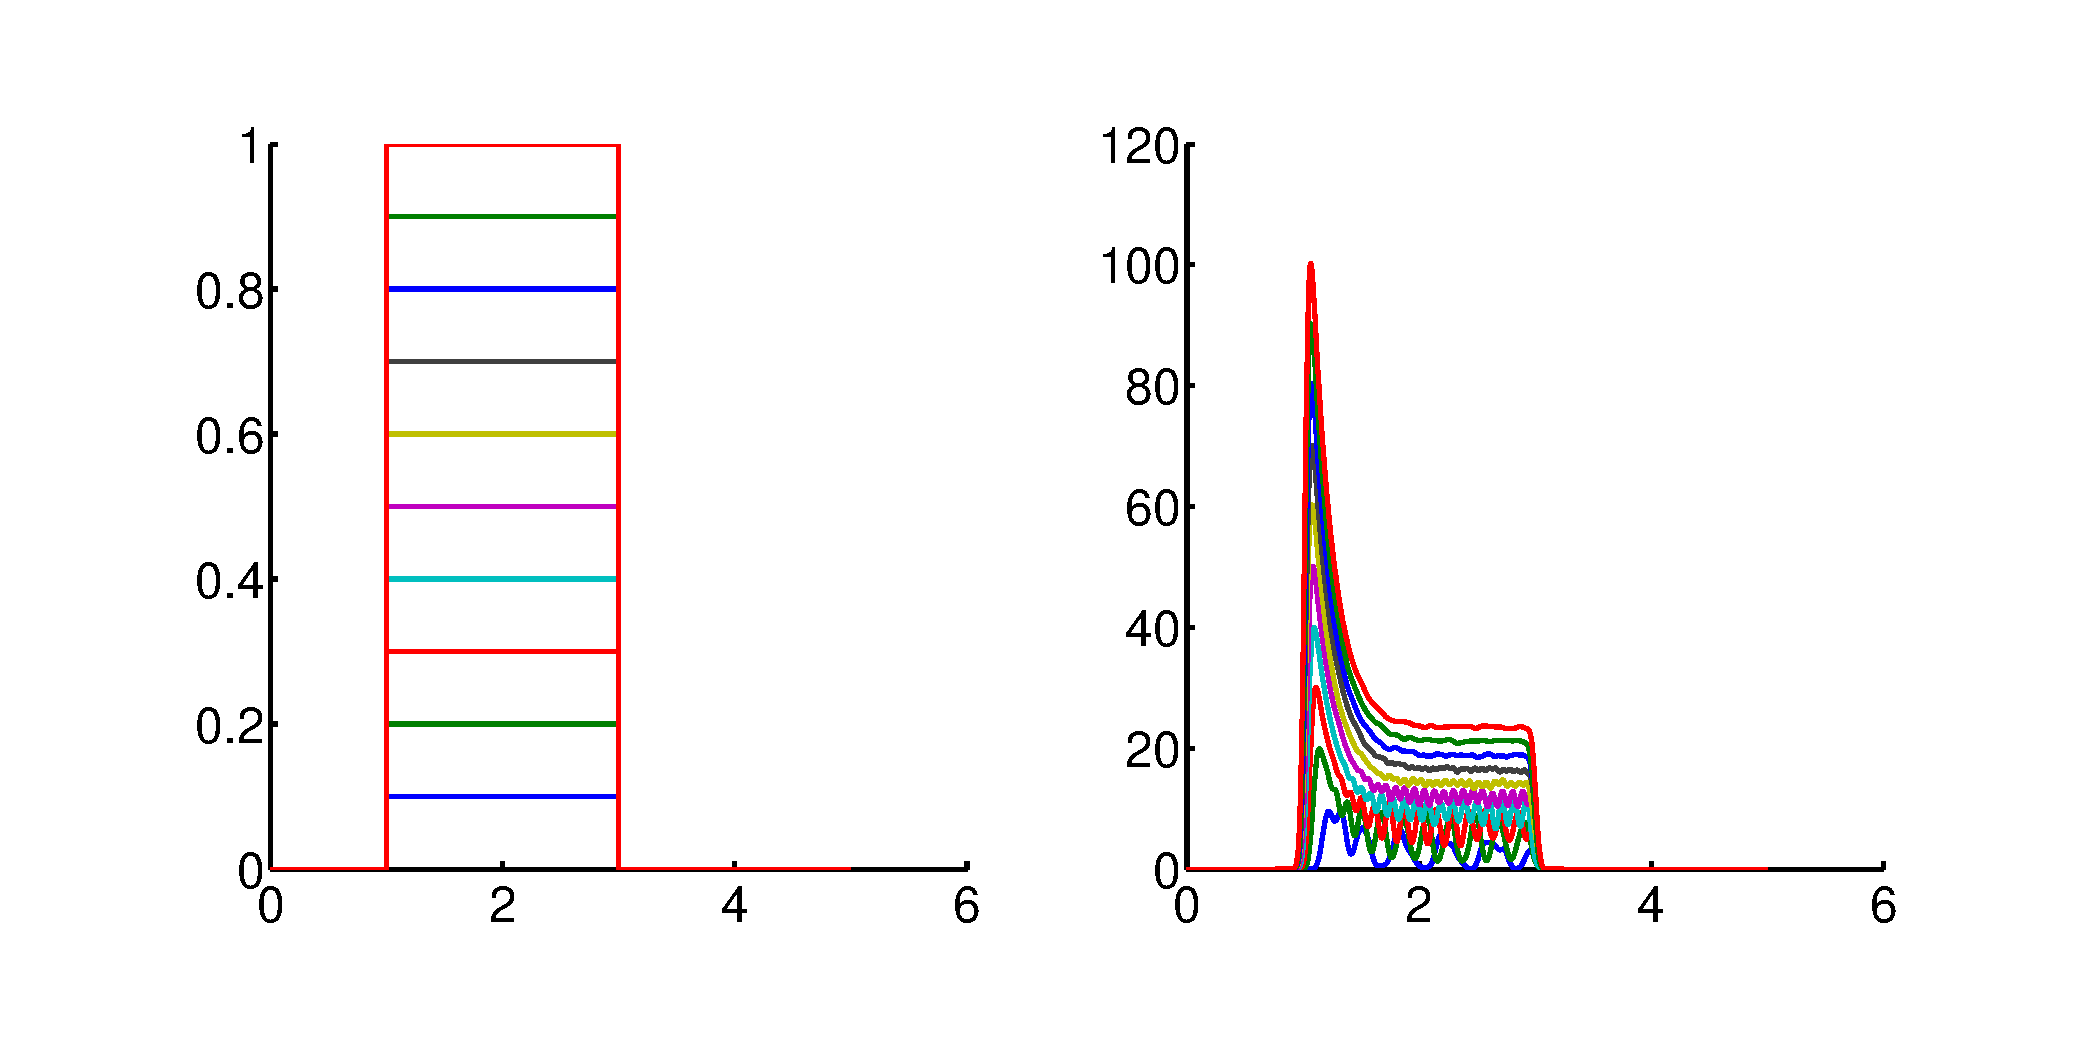
\includegraphics [width=\textwidth]{SpikeFreqAdaptation_01.pdf}


\subsection*{Response to exponentiated Gaussian stimuli}

\begin{par}
Now we simulate some flickering stimuli by exponentiated Gaussian noise and use that to feed the neuron. The following figure shows the output of the model neuron, together with a linear fit to the model output.
\end{par} \vspace{1em}

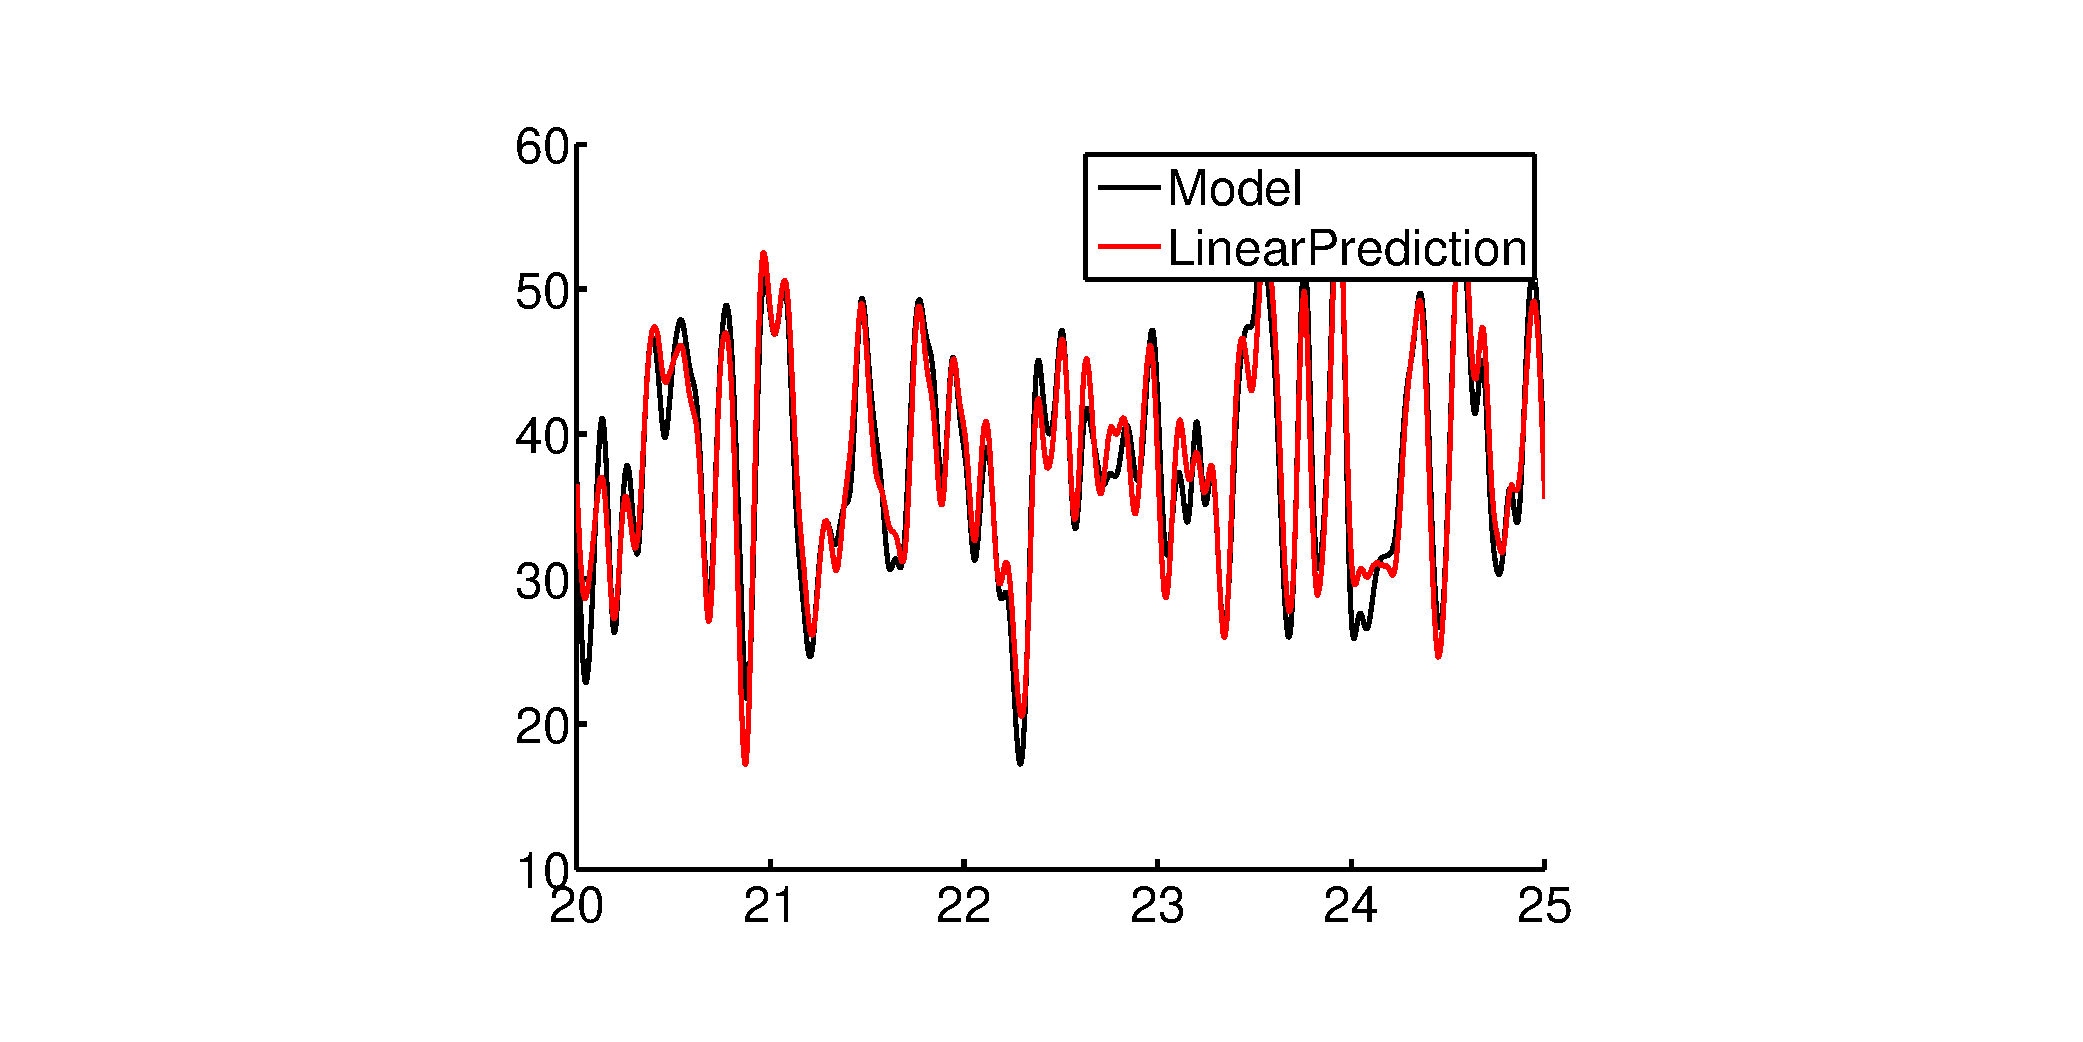
\includegraphics [width=\textwidth]{SpikeFreqAdaptation_02.pdf}


\subsection*{Does this show the signature of fast adaptation?}

\begin{par}
Does the (feedback) mechanism of spike frequency adaptation allow the neuron to modulate its gain on a fast time scale, like in real ORNs? We perform a linear gain analysis as before.
\end{par} \vspace{1em}

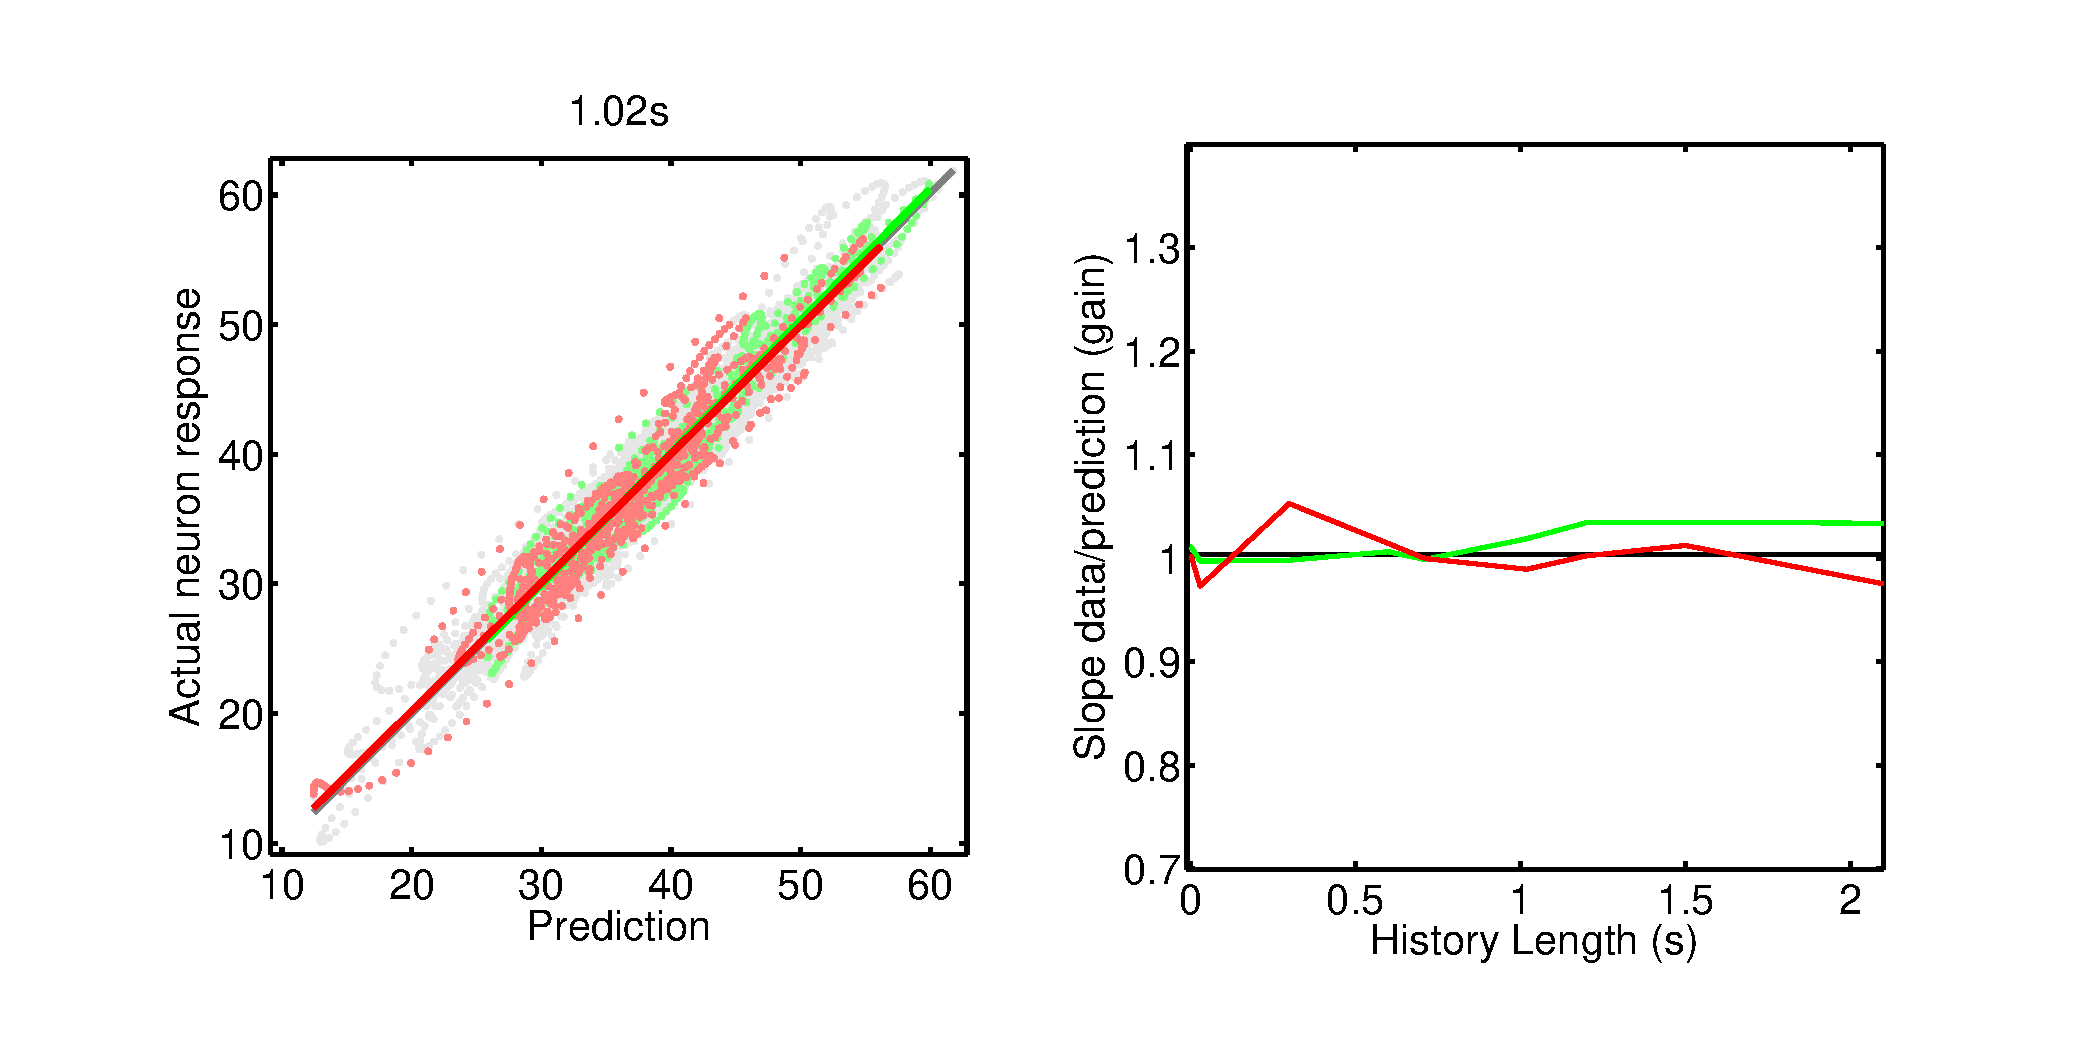
\includegraphics [width=\textwidth]{SpikeFreqAdaptation_03.pdf}



\end{document}
    
